The contribution of this dissertation is a coherent collection of novel data structures and algorithms for integration and interactive visualization of many data sets from multiple sources, based on the data cube concept. The proposed data representation framework will allow data sets to be combined together and visualized using interactive visualization dashboards, giving users the sense that the data exists within a single unified structure. The framework is designed to be able to represent and integrate an arbitrary number of data sets created independently of one another, and expose the integrated structure to reusable visualizations. The reusable visualizations can be combined together in dashboard layouts with multiple linked views using existing interaction techniques such as brushing and linking. The proposed data representation and visualization framework is fundamentally new, and will allow heterogeneous data sets to be explored in a unified way that was never before possible. 

\section{Vision}
The overall goal of this work is to build digital telescope into the universe of phenomena on Earth via publicly available data. For example, consider public data sources such as the United Nations, the US Census, the US Bureau of Labor Statistics, or the US Centers for Disease Control. These organizations and hundreds of others around the world provide publicly available data about various topics including population statistics, public health, distribution of wealth, quality of life, economics, the environment, and many others. By unifying these data sources and providing users with tools to explore and present the data visually, a deeper understanding of the world can be gleaned through the lens of public data. The focus of this dissertation is on applications involving public data, however the techniques introduced can be applied to any data sets that can be conceptually modeled as data cubes, regardless of whether they are public or private. 

Consider the data from the US Census that covers population statistics for US States from 1950 to 2010. Consider also population statistics from the United Nations covering World Countries from 1970 to 2012. These two data sets may use different identifiers for years and geographic regions, but they cover an overlapping conceptual data space of time, geography and population. From these two data sets it is possible to create a visualization dashboard with a map of the world showing population as color and a corresponding line graph showing population for each region as lines.

If the user views the whole world, the UN population data is shown for each country. If the user zooms into the US, US Census data is shown for each state. If the user selects a point of time in the line graph, the data shown on the map is from that point in time. If the user pans and zooms on the map, the lines in the line graph update to only show the regions visible on the map. This is one example of an interactive visualization dashboard with multiple linked views (the timeline and map views) operating over multiple data sets integrated from different sources (the United Nations population data and the US Census population data).

\begin{figure}[h]
  \caption{An example visualization dashboard with multiple linked views. Selecting a time on the line chart slices the data displayed on the choropleth map. Zooming and panning on the choropleth map filter the country profiles shown in the line chart. The vertical black line on the line chart indicates the selected year.}
  \centering
  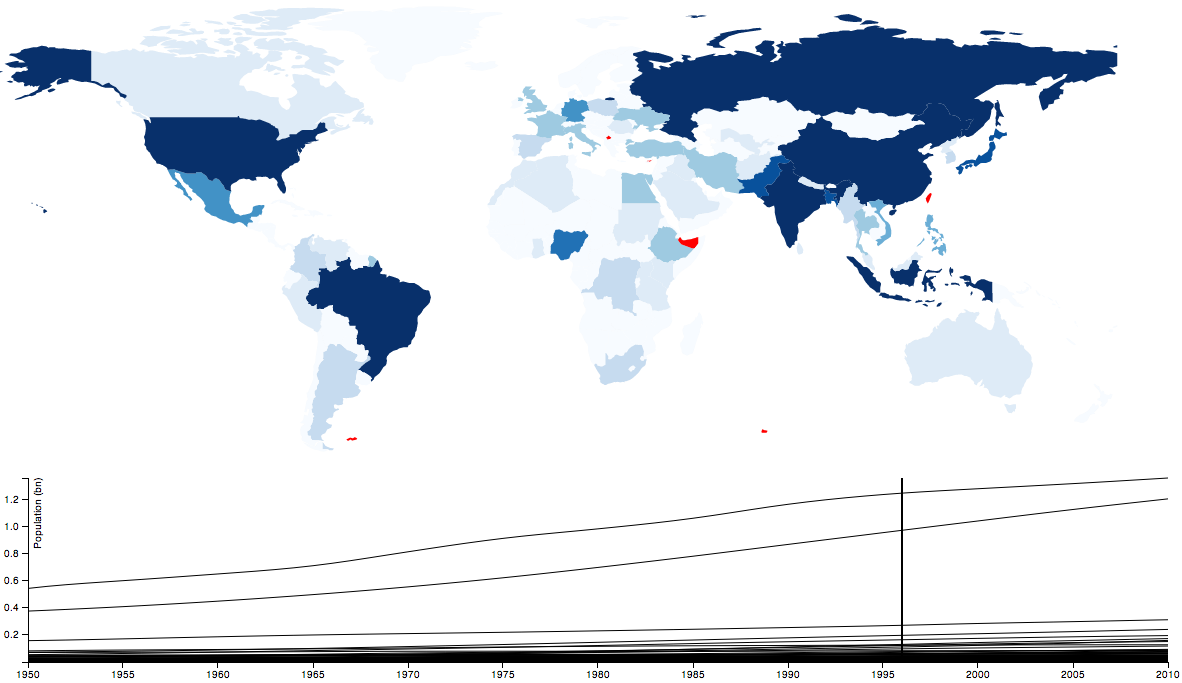
\includegraphics[width=\textwidth]{figures/linkedChoropleth.png}
\end{figure}

\TODO{Improve this visualization - add color legend, add names to lines}

Data cubes, also known as OLAP (OnLine Analytical Processing) cubes, can represent data that contains measures aggregated (typically using sum or average) along categorical hierarchies. The data cube concept emerged from the field of data warehousing as a way to summarize transactional data, allowing analysts to get a bird's eye view of company activities. The term OLAP stands in contrast to the term OLTP (OnLine Transaction Processing), which is the part of the data warehouse system that ingests and stores data at the level of individual transactions or events. After the ETL (Extract, Transform and Load) phase of the data warehouse flow, the data is analyzed by computing a data cube from the transactional data.

The data cube concept and structure can be used to model existing data sets as well. Publicly available data sets (often termed ``statistical data'') may be considered as pre-computed data cubes if they contain aggregated measures (also called ``indicators'', ``metrics'' or ``statistics'') across time, geographic space or other dimensions such as gender, age range, ethnicity or industry sector. Any categorization scheme containing distinct entities, organized as an unorered collection, an ordered collection, or a hierarchy can be modeled as a dimension. Any numeric value that represents an aggregated statistical summary using sum, average, or other aggregation operator can be modeled as a measure.

With this approach, it is possible to model many data sets together using shared dimensions and measures. This allows integration of many data sets together in a single unified structure. Existing data cube technologies assume that data cubes will be computed from a relational source, and are not designed to handle integration of pre-computed data cubes that may use inconsistent identifiers for common dimensions and inconsistent scaling factors for common measures. Therefore the application of the data cube concept to integration and visualization of many pre-computed data cubes, while theoretically plausible, requires the development of novel data structures and algorithms that extend the data cube model to handle integration of pre-computed data cubes that may use inconsistent identifiers for common dimensions and inconsistent scaling factors for common measures.

The data cube structure lends itself particularly well to visualization. Long standing data visualization theory presented by Bertin \cite{bertin1983semiology} and Mackinlay \cite{mackinlay1986automating} identify effective ways to visually encode data based on data fields that are nominal, ordinal or quantitative. Visualization and interaction techniques have been explored for hierarchical (tree-based) data as well \cite{graham2010survey, yang2003interactive}. Data cubes can contain data of all these types (dimensions can be nominal, ordered, or hierarchical; measures are quantitative). Therefore existing visualization theory can be applied to the data cube model to determine which visualizations are appropriate for representing which data, depending on its data cube structure.

\pagebreak
\section{Related Work}
Previous work relating to this dissertation falls into four major categories:
\begin{itemize}
\item data representation - structures, models and formats for data
\item data integration - merging data from many sources
\item data visualization - transforming data into interactive graphics
\item Web graphics technology - HTML5 graphics APIs and libraries
\end{itemize}
\subsection{Data Representation}
In today's world of ``information overload'', data takes many forms. Perhaps the most familiar data representation system today is Microsoft Excel, which is capable of representing data tables as well as complex operations across the data values. Many organizations use Excel to manage data or make data available as Excel spreadsheets. For example, the United Nations Department of Economic and Social Affairs makes their population statistics available in Excel format (see figure \ref{fig:unPopExcel}). Many data tables on the Web are made available in simpler text-based formats such as CSV (Comma Separated Values) or TSV (Tab Separated Values). Data sets are also frequently made available in proprietary formats that may be text based or binary, such as ESRI Shapefiles or Adobe PDF documents.

\begin{figure}[h!]
  \centering
  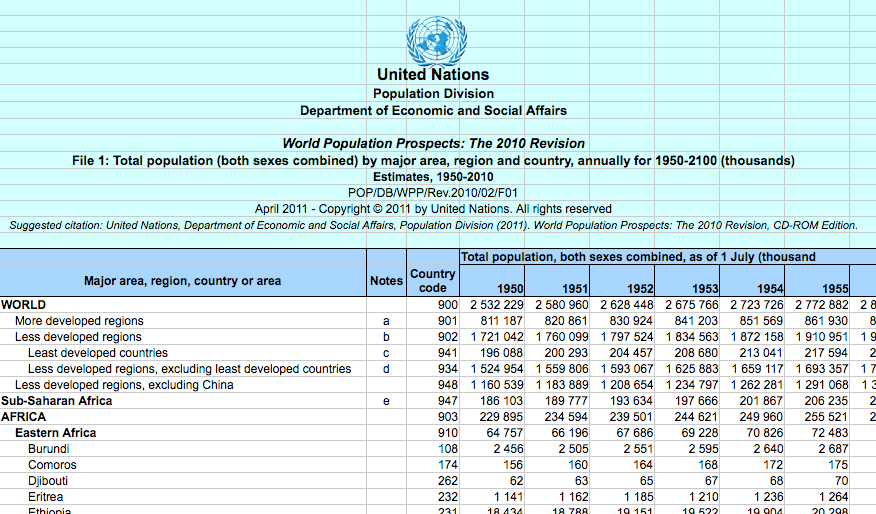
\includegraphics[width=\textwidth]{figures/UN_World_Population_Spreadsheet.png}
  \caption[United Nations population estimates spreadsheet.]
   {The United Nations Population Prospects data set \cite{unPopData}, made available in Excel format. This is an example of a public data set that can be imported into our data representation framework.}
  \label{fig:unPopExcel}
\end{figure}

Relational database systems provide a mature data management solution and are widely adopted \cite{ramakrishnan2000database}. The relational model has well understood theoretical underpinnings such as relational algebra \cite{clifford1985algebra}. Data warehouse systems are typically built on the relational model and are augmented by multi-scale aggregated data structures called data cubes, also known as OLAP (OnLine Analytical Processing) cubes \cite{gray1997data, codd1993providing}. Data cubes contain summaries of the collection of facts stored in a relational database \cite{chaudhuri1997overview}. For example, a data cube may contain how much profit was made from month to month subdivided by product category, while the relational database may contain the information associated with each individual transaction.

Because data cubes provide an abstraction that handles aggregation, they are a widely used method of data abstraction for supporting visualization and analysis tasks \cite{stolte2003multiscale}. Kimball pioneered the area of ``Dimensional Modeling'', which concerns constructing data warehouse schemas amenable to data cube construction and analysis \cite{kimball1998data}. Data cubes have been implemented in a variety of different systems, so effort has been made to discover unified conceptual or mathematical models that can characterize many implementations \cite{datta1999cube, vassiliadis1999survey, vassiliadis1998modeling, li1996data, agrawal1997modeling, gyssens1997foundation, blaschka1998finding}. The data cube structure has also been used to model user Web browsing sessions to support data mining algorithms for Web prefetching \cite{yang2003data}.
%
%NoSQL systems are modern databases that are designed to go beyond the scalability limitations of relational systems \cite{cattell2011scalable}. While NoSQL systems sacrifice some of the integrity constraints upheld by relational database systems \cite{stonebraker2010sql}, they are gaining traction in industry because they can handle the scale of data demanded by applications of the ``Big Data'' era \cite{leavitt2010will}. NoSQL systems provide flexible storage systems that do not necessarily require the definition of a schema. This makes it arguably easier to modify and update the type of content stored over time as compared to relational systems.
%
%The Semantic Web is a vision of a ``Web of Data'' coexisting with the World Wide Web \cite{berners2001semantic}. The basis of the Semantic Web is the RDF (Resource Description Framework) data model, which represents a graph of data in the form of (subject, predicate, object) triples. The Semantic Web vision has evolved into the concept of Linked Data, which refers to data that is available as RDF and made available according to common conventions \cite{bizer2009linked} \cite{bizer2007publish}. Any data that can be represented using a relational database can also be represented using RDF \cite{bizer2006d2r}. The SPARQL query language for RDF can be used to query and integrate data from multiple sources \cite{quilitz2008querying}. Lopez et al. developed an information management system for integrating and analyzing heterogeneous information sources characterizing urban areas \cite{lopez2012queriocity}. The Semantic Web technology stack contains a method for declaring when different identifiers refer to the same entity and processing queries appropriately to integrate data \cite{halpin2010owl} \cite{ding2010sameas}. While the Semantic Web provides a compelling vision, its adoption is not as widespread as one might expect \cite{lytras2008semantic}.
%
%The RDF Data Cube Vocabulary is capable of representing data cubes using Semantic Web technologies \cite{rdfdatacube}. The intention of the RDF Data Cube Vocabulary is to provide a common representation and interchange format for statistical data. The RDF Data Cube Vocabulary draws from a previous effort called the Statistical Data and Metadata eXchange (SDMX) initiative that was launched in 2001 by seven organizations working on statistics at the international level \cite{cyganiak2010semantic}. The primary challenges faced when using the RDF Data Cube Vocabulary include transforming to and from well known formats and data models. Salas et al. discussed how data can be transformed from existing OLAP systems or flat files into RDF using the Data Cube Vocabulary, and also introduced a faceted visualization tool for RDF data cubes \cite{salas-icsc-2012}. K{\"a}mpgen et al. investigated how data represented using the RDF Data Cube Vocabulary can be transformed for analysis using traditional OLAP systems \cite{kampgen2011transforming}. Maali et al. proposed a pipeline for converting government data into high quality Linked Data utilizing the Data Cube Vocabulary \cite{maali2012publishing}.
%
%Datta et al. introduce a conceptual model for data cubes \cite{datta1999cube}. In this formalization, a data cube (or, in the terms of the authors, a data cube instance) is defined as a 6-tuple $(D, M, A, f, V, g)$ where $D$ is a set of dimensions, $M$ is a set of measures, $A$ is a set of attributes, $f$ is a function that maps dimensions to sets of attributes (the levels of the dimension), $V$ is a set of tuples that assign concrete numeric values for each measure, and $g$ is a function that maps data cube cells to tuples in $V$. The authors formalize common OLAP operators including slice, drill-down, roll-up, and pivot, as well as operators over multiple cubes including join, union, intersection and difference. This formalism captures the essence of data cubes, but is limited in that it does not deal with integrating data cubes from multiple sources where names used for dimensions, attributes and measures may not match.
%
%Kuznetsov et al. introduce a mathematical formalism of data cubes based on lattice theory \cite{kuznetsov2009mathematical}. This work focuses primarily on characterizing the lattice structure of hierarchical data cubes and relating the structure to established mathematics in lattice theory. The contribution of this work is primarily mathematical, and the structures introduced do not cover the entire problem area of representing, structuring and querying complete data cubes. This characterization is similar to the zoom graph concept introduced by stolte et al. \cite{stolte2003multiscale}. Usman et al. introduced a conceptual model for OLAP enhanced for coupling with data mining and visualization techniques \cite{usman2009conceptual}.
%
\subsection{Data Integration}
The field of data integration offers many techniques for combining data from multiple sources based on the relational model \cite{doan2012principles} as well as from a theoretical perspective \cite{lenzerini2002data, halevy2006data, ziegler2004three}. Schema matching is the area of data integration that concerns semantic matching between the attributes of data tables from different sources \cite{rahm2001survey, fagin2003data}. Schema matching may be performed manually, however it must be automated in order to scale to hundreds or thousands of different sources. Numerous approaches for automated schema matching have been proposed \cite{shvaiko2005survey, doan2001reconciling, kang2003schema, milo1998using, madhavan2001generic, doan2000learning}. Schema matching approaches aimed specifically at Web and Ontology based data integration have also been proposed \cite{he2003statistical, noy2004semantic, doan2005semantic, madhavan2007web, kalfoglou2003ontology, noy2009ontology, uschold2004ontologies, wache2001ontology, noy2003prompt, euzenat2007ontology}. Data matching (also known as record linkage) is the area of data integration focusing on resolving different identifiers to the same real-world entity \cite{winkler1999state, winkler2006overview, koudas2006record, aizawa2005fast, gu2003record, winkler1995matching}. Record linkage has been applied extensively to public data \cite{jaro1995probabilistic, jaro1989advances, holman1999population}. Several tools have been introduced that aid users in data integration tasks via a graphical user interface \cite{christen2008febrl, kandel2011wrangler, elfeky2002tailor}.

\subsection{Data Visualization}
The field of information visualization offers many compelling approaches for visualizing data \cite{keim2002information}. Arguably the first significant work concerning data visualization was William Playfair's ``Commercial and Political Atlas'', published in 1786 \cite{playfair1786commercial}. In this work, Playfair introduced the Bar Chart, Pie Chart, and Line Graph. The first attempt at a systematic formalization of data visualization was Jacques Bertin's ``Semiology of Graphics'' \cite{bertin1983semiology}. In this work, Bertin relates data types to visual marks and channels in a coherent system that takes visual perception into account. Bertin's work has influenced many future theoretical underpinnings of visualization, including Leland Wilkinson's ``Grammar of Graphics'' \cite{wilkinson2005grammar} and Jock Mackinlay's APT (A Presentation Tool) system \cite{mackinlay1986automating}.

Interactive data visualization systems based on straightforward tables are plentiful. Tableau is a commercial visualization package supporting creation of interactive visualization dashboards \cite{hanrahan2007visual}. Spotfire is a framework for constructing information visualization systems \cite{ahlberg1996spotfire}. GGobi is an extensible framework (based on XGobi) for interactive data visualization based on the R platform \cite{swayne2003ggobi, swayne1998xgobi}. Gee et al. presented the Universal Visualization Platform, a general interactive visualization infrastructure upon which others can build knowledge discovery applications. North et al. introduced Snap-Together Visualization, a user interface for coordinating visualizations \cite{north2000snap} and an extension of the architecture for the Web \cite{north2002visualization}. Fekete introduced the InfoVis Toolkit, a collection of reusable visualization components. GeoDa is a tool for interactive visual exploration of multidimentional data with a geospatial component \cite{anselin1999interactive}. 

Much effort has been placed on generating taxonomies of visualization techniques. Chi et al. introduced a taxonomy of visualizations based on the Data State Reference Model \cite{chi2000taxonomy, chi1998operator}. Shneiderman introduced a more general taxonomy based on tasks and data types \cite{shneiderman1996eyes}. Card et al. made steps toward characterizing the entire design space of data visualizations based on Bertin's theory \cite{card1997structure}. Tufte explored numerous visualization techniques for quantitative information in general, many of which can be applied to visualization of data cubes \cite{tufte1983visual}.

Much work has been done regarding visualization of data cubes. Stolte et al. introduced a formalism for defining multi-scale visualizations of data cubes throughout their work on the Polaris system \cite{stolte2003multiscale, stolte2002query, stolte2002polaris}. In this work the authors introduce theoretical underpinnings of a visualization system capable of navigating hierarchical data cubes with a combination of data abstraction and visual abstraction. Eick introduced the ADVISOR system, which focused on visualizing data cubes and categorizing classes of data cube visualizations \cite{eick2000visualizing}. Eick discussed the following ``perspectives'' of data cube visualizations: Single Measure, Multiple Measures and Anchored Measures. He also discussed the following interaction techniques for data cube visualizations: Undo and Redo, Bookmarks, Selection (Replace, Intersect, Add, Subtract, Select All, Unselect All, Toggle), and Exclusion.

Mansmann coined the term ``Visual OLAP'', framed it as a fundamentally new paradigm for exploring multidimensional aggregates \cite{mansmann2008visual}, explored applications of hierarchical visualization techniques to OLAP cubes \cite{mansmann2007exploring} and extended Visual OLAP to support irregular hierarchies \cite{mansmann2006extending}. Cuzzocrea et al. surveyed the area of data cube visualization in depth \cite{cuzzocrea2009olap} and have made several contributions regarding semantics-aware OLAP visualization \cite{cuzzocrea2007semantics} and a hierarchy driven compression technique for OLAP visualization \cite{cuzzocrea2006hierarchy}. Scotch et al. developed and evaluated SOVAT, a Spatial OLAP visualization and analysis tool applied to community health assessments \cite{scotch2005sovat, scotch2007usability}. Lee and Ong introduced a visualisation technique for knowledge discovery in OLAP combining elements of bar charts and parallel coordinates \cite{lee1995new}. Maniatis et al. explored how OLAP cubes can be visualized using TableLens and other techniques \cite{maniatis2003advanced}. Data cubes have also been utilized as the foundational data structure for several ``Big Data'' visualization systems \cite{lins2013nanocubes, liu2013immens}.

Interactions within data visualization environments have been well studied. Becker et al. investigated brushing in scatter plots \cite{becker1987brushing}. Shneiderman et al. explored dynamic queries in general and how these operations fit into a larger context of visual information seeking \cite{shneiderman1994dynamic}. Ward introduced a visualization system based on multiple linked views with direct manipulation techniques including brushing and linking \cite{ward1994xmdvtool}. Anselin discussed how interactive visualization systems with linked views can be applied to Geographic Information Systems \cite{anselin1999interactive}. Yi et al. conducted a thorough survey of existing taxonomies for visualization and interactions and developed a set of generalized classes of interactions for visualization \cite{yi2007toward}. Techapichetvanich et al. explored how visualization interactions pertain to OLAP cubes in particular \cite{techapichetvanich2005interactive}. Sifer et al. introduced a visual interface utilizing coordinated dimension hierarchies for OLAP cubes \cite{sifer2003visual}. Tegarden formulates some requirements for information visualization relevant for business applications, and highlights some unconventional interactive visualizations with potential application to data cube visualization \cite{tegarden1999business}.

\subsection{Web Graphics Technology}
The World Wide Web has evolved to become a full fledged application development platform \cite{pilgrim2010html5}. HTML5 is the latest set of standards and APIs (Application Programming Interfaces) from the World Wide Web Consortium that define the capabilities of modern Web browsers \cite{html5}. HTML5 contains three graphics technologies that can support interactive Web-based visualizations: Canvas, SVG (Scalable Vector Graphics), and WebGL.

HTML5 Canvas provides a 2D immediate mode graphics API \cite{fulton2013html5}. When using the Canvas API, developers must work with a stateful graphics context by issuing commands to manipulate the raster image of a Canvas element within the HTML page. This approach requires developers to manage rendering logic at a low level and manage data structures that correspond to graphical representations. The Canvas API has seen wide adoption for HTML5-based games, however for visualization applications the higher level SVG API has seen wider adoption.

SVG (Scalable Vector Graphics) provides a 2D retained mode Graphics API \cite{svg}. SVG uses the HTML DOM (Document Object Model) to represent the definition of persistent graphical elements. When using SVG, developers need only be concerned with updating the DOM. The SVG engine within the browser is responsible for updating the display to correspond with the SVG DOM. In this way, SVG is a higher level API than Canvas. This makes SVG a preferred platform for developing visualizations. However, SVG is less optimizable than Canvas, because developers do not have access to the rendering logic. SVG has performance limitations relating to DOM manipulation overhead.

WebGL provides a 3D graphics API that is essentially a JavaScript interface to OpenGL ES \cite{matsuda2013webgl}. OpenGL ES is a subset of OpenGL designed for use in embedded systems and mobile devices. Developers using WebGL must use programming techniques inherited from OpenGL such as buffer management, vertex management, shader definition, 3D projection, and lighting techniques. WebGL enables developers to take advantage of the GPU (Graphics Processing Unit) for massively parallel computation using shaders. WebGL supports high performance 2D and 3D graphics, but is much more complicated to use than Canvas or SVG. WebGL has been applied to interactive visualization of volumetric data \cite{congote2011interactive}.

Many high level libraries have been built for supporting use of Web graphics technologies. Three.js is a 3D scene graph library that includes rendering engines for all three graphics technologies \cite{cabello2010three}. Highcharts is a high level visualization library that provides pre-packaged chart types that can be customized to a limited extent. Leaflet is a library for creating tile-based geographic maps with zooming and panning. hBrowse is a generic framework introduced for Web-based hierarchy visualization \cite{kokoszkiewicz2012hbrowse}. Processing.js is a JavaScript port of the graphics language Processing using HTML5 Canvas. Many more libraries for Web-based graphics and visualization exist, but none have come close to the widespread adoption of D3.js.

D3.js is a flexible and powerful visualization library that uses SVG and has a strong community of users \cite{d3}. D3 at its core is a DOM manipulation library with heavy use of functional programming. D3 allows concise declarative statements to define the core logic of visualizations. D3 provides additional APIs for performing common visualization tasks such as defining and using scales, generating labeled axes, and computing layouts from graphs and trees. D3 is at the center of a vibrant developer ecosystem and has seen wide adoption in industry. There are plentiful examples of D3.js usage for creating visualizations. Many supporting libraries for D3 have been created including Chart.js for composing visualization elements, Crossfilter.js for interactive multidimensional filtering, and DC.js for multiple linked views. Several reusable D3 chart libraries have appeared including NVD3, reD3, and dimple.

%\begin{figure}[h!]
%  \centering
%  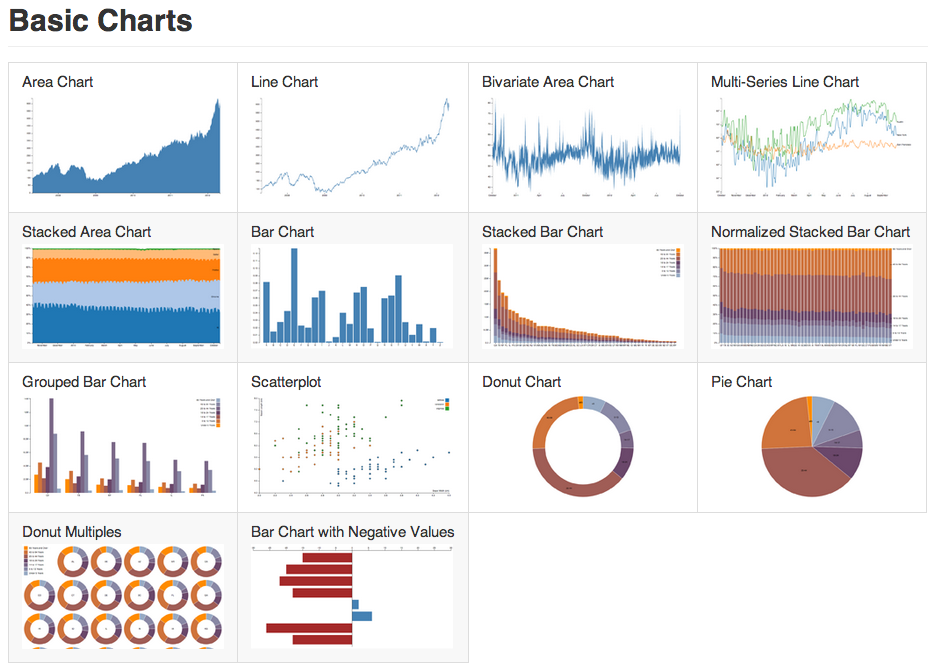
\includegraphics[width=\textwidth]{figures/d3BasicCharts.png}
%  \caption[D3.js basic charts.]
%    {Basic chart examples using D3.js. These are some examples of visualizations that can be tailored to visualize and interact with data cube projections in a generalized manner, building on our proposed framework.}
%  \label{fig:d3basic}
%\end{figure}
%
Several projects have focused explicitly on visualization of public data on the Web. ManyEyes was an experiment in scaling the audience for visualizations by empowering users to create visualizations of their own data \cite{viegas2007manyeyes}. ManyEyes provided a fixed set of pre-packaged visualization tools and allowed users to visualize their own data tables using the provided visualizations. GapMinder is a project aimed at exposing public data (primarily the United Nations Millenium Development Goals Indicators) using visualization \cite{rosling2005new}. GapMinder includes an animated scatter plot with an interactive time slider, a line chart showing statistics over time, and a world map. The Google Public Data Explorer provides a visual interface to selected public data sets similar to GapMinder, however it does not make the data available to users in a machine-readable format.

%\begin{figure}[h!]
%  \centering
%  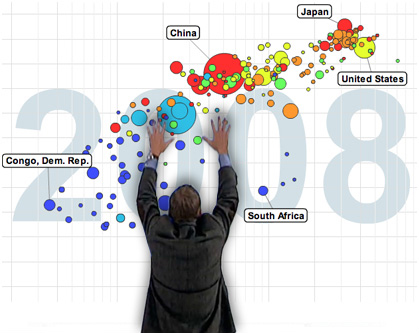
\includegraphics[width=\textwidth]{figures/gapminder.jpg}
%  \caption[GapMinder and Hans Rosling.]
%   {Gapminder, a public data visualization tool based on an animated scatter plot, timeline, and map. Here, Professor Hans Rosling, the creator of GapMinder, is shown gesturing the motion of the plot while presenting the visualization.}
%  \label{fig:gapminder}
%\end{figure}

\section{Pseudocode Conventions}
Throughout this document, pseudocode is used to express data structures and algorithms. Our pseudocode is similar to that found in the book ``Introduction to Algorithms'' \cite{cormen2009introduction}, but differs significantly in that it uses a functional style. Primitive types in our pseudocode include numbers, strings, booleans, arrays, objects and functions. The following examples demonstrate the features of our pseudocode language.

\subsection{Operators and Primitive Types}

\begin{codebox}
\li $x \gets 5$
\end{codebox}

Line numbers appear to the left of each line of pseudocode. Variables can have any name comprised of characters without spaces, and can be assigned a value with the $=$ symbol. Variables need not be explicitly declared. The scope of a variable is determined by where it is first assigned. Our pseudocode uses block scope, meaning that every indentation level introduces a new nested scope. On line 1 of the above pseudocode example, the variable $x$ is defined and assigned the value of $5$, a numeric literal.

The following pseudocode demonstrates numbers, strings and booleans.

\begin{codebox}
\li $myNumber \gets 5$
\li $myString \gets $ \verb1'test'1
\li $myBoolean \gets \const{true} $
\li $myOtherBoolean \gets \const{false} $
\end{codebox}

All numbers are treated as double precision floating point. Numeric literals in pseucode become numbers (see line 1). String literals are denoted by single quotes and a monospace font (see line 2). Booleans can be either true or false. True and false are builtin constant boolean values denoted by all capitalized words (see lines 3 and 4). Camel case names starting with a lower case letter are used for most variables in our pseudocode.

\subsection{Functions}
\begin{codebox}
\li $add \gets \lambda(a, b)$
\Do
\li \Return $ a + b $
\End
\li $result = add(4, 6)$ \Comment $result$ is assigned the value $10$
\li $triple \gets \lambda(x)$ \Return $ x * 3 $
\li $triple(3)$ \Comment evaluates to $9$
\end{codebox}

The above pseudocode demonstrates how a function is defined and invoked, and also introduces comments. This example defines a function called $add$ (on lines 1 and 2) that adds two numbers together. The $\lambda$ (lambda) symbol defines a new anonymus function. Variables can be assigned functions as values using $=$. The comma separated names in parentheses directly following the $\lambda$ are the arguments to the function. The pseudocode on lines following the $\lambda$ that is indented one level constitutes the function body (also called the function closure). The function arguments are only visible inside the function closure.

Functions can be invoked using parentheses. The argument values are passed to the function in a comma separated list within parentheses. On line 3, the $add$ function is invoked, passing the value $4$ as argument $a$ and $6$ as argument $b$. The value returned by the function is assigned to the variable $result$. The function invocation causes the function body to execute, which adds the two numbers together and returns the resulting number using the ``return'' keyword on line 2. Lines 4 and 5 demonstrate that a simple anonymous function can be defined in a single line. Text following the $//$ symbol is a comment, and is not executed.

\subsection{Arrays}
\begin{codebox}
\li $myArray \gets [\,]$ \label{emptyArrLiteral}
\li $myArray.push(5)$ \Comment $myArray$ now contains $[5]$ \label{beginArrPush}
\li $myArray.push(7)$ \Comment $myArray$ now contains $[5, 7]$
\li $myArray.push(9)$ \Comment $myArray$ now contains $[5, 7, 9]$ \label{endArrPush}
\li $myArray[0]$ \Comment evaluates to $5$
\li $myArray[2]$ \Comment evaluates to $9$
\li $myArray[1] = 3$ \Comment $myArray$ now contains $[5, 3, 9]$
\li $myBooleanArray \gets [\const{true}, \const{false}, \const{true}, \const{true}]$ \label{arrLiteral1}
\li $myStringArray \gets [$\verb1'foo'1$,$\verb1'bar'1$]$ \label{arrLiteral2}
\li $numberOfBooleans \gets myBooleanArray.length$ \Comment evaluates to 4 \label{arrLenBegin}
\li $numberOfStrings \gets myStringArray.length$ \Comment evaluates to 2 \label{arrLenEnd}
\li \For $str \in myStringArray$ \label{forLoop1}
\Do
\li   $log(str)$ \Comment prints \verb1'foo'1 then \verb1'bar'1 \label{forLoop2}
\End
\li $myArray.map(triple)$ \Comment evaluates to $[15, 21, 27]$ \label{arrMap}
\end{codebox}

The above pseudocode demonstrates arrays. Arrays are ordered lists of elements. Arrays can contain elements of any type. Array literals are denoted by square brackets and can be empty (as in line \ref{emptyArrLiteral}) or populated (as in lines \ref{arrLiteral1} and \ref{arrLiteral2}). Arrays have a built-in function attached to them called $push$, which appends a new element to the end of the array. Lines \ref{beginArrPush}-\ref{endArrPush} demonstrate how $push$ can be used to append items to an array. The dot notation seen on lines \ref{beginArrPush}-\ref{endArrPush}, \ref{arrLenBegin}-\ref{arrLenEnd} and \ref{arrMap} is used on arrays only to access the following built-in array functions and properties.

\begin{itemize}
\item $length$ the number of items in the array
\item $push(item)$ appends an item to the end of an array
\item $map(callback)$ calls $callback(item)$ for each $item$ in the array
\end{itemize}

Square brackets denote access of array elements by index when placed directly after the array variable. Lines 5 and 6 demonstrate how square bracket notation can be used to access values in an array based on their index. Line 7 demonstrates that square bracket notation can also be used to assign to values in an array. Lines 10 and 11 demonstrate the built-in property $length$, the number of elements in the array. Array indices start at zero. 

Line \ref{forLoop1} introduces the for loop construct. A for loop iterates over each element in the array. The indented code block following the for loop construct is executed once for each item in the array. In this example, each item is bound to the variable $str$, which is only visible within the for loop body. Line \ref{forLoop2} invokes the built-in function $log(message)$, which prints out the message passed into it to.

Line \ref{arrMap} introduces the map construct. The built-in $map(iterator)$ function applies the given $iterator(item)$ function to each item in the array, and returns a new array populated with the returned values from $iterator$. In this example, the function $triple$ defined earlier is applied to each element in the $myArray$ array, yielding a new array with all values tripled.

\subsection{Objects}\label{objects}
\begin{codebox}
\li $myObject \gets \{\,\}$ \label{emptyObject}
\li $myObject.first = $\verb1'John'1 \Comment $myObject$ now contains $\{first:$\verb1'John'1$\} $ \label{dotAssignment}
\li $myObject[$\verb1'last'1$] = $\verb1'Doe'1 \Comment now $\{first:$\verb1'John'1$, last:$\verb1'Doe'1$\}$ \label{bracketAssignment}
\li $myOtherObject = \{first:$\verb1'Jane'1$, last:$\verb1'Doe'1$\}$ \label{singleLineObjectLiteral}
\li $box = $ \label{beginMultiLineOblectLiteral}
\Do
\li   $x: 50$
\li   $y: 60$
\li   $width: 100$
\li   $height: 150$ \label{endMultiLineObjectLiteral}
\End
\li $keys = keys(box)$ \Comment evaluates to $[$\verb1x1$,$\verb1y1$,$\verb1width1$,$\verb1height1$]$ \label{objectKeys}
\li $values = keys.map(\lambda(property) \; \Return \; box[property])$ \label{extractProperties}
\li \Comment $values$ is assigned $[50, 60, 100, 150]$
\li $box[$\verb1'nonexistentProperty'1$]$ \Comment evaluates to \const{nil} \label{nil}
\end{codebox}

The above pseudocode introduces objects. Objects are key-value mappings (sometimes called \emph{maps} or \emph{dictionaries}). Curly braces denote single-line object literals. Line \ref{emptyObject} assigns the variable $myObject$ to an empty object. Object properties can be assigned using dot notation, as in line \ref{dotAssignment}, or square bracket notation, as in line \ref{bracketAssignment}. Bracket notation is useful when the property name is stored as a string in a variable. Object literals can contain key-value pairs denoted by $key: value$ as in line \ref{singleLineObjectLiteral}. When an object literal spans multiple lines, the curly braces are omitted and the key-value pairs are indented, as in lines \ref{beginMultiLineOblectLiteral}-\ref{endMultiLineObjectLiteral}. Line \ref{objectKeys} introduces the built-in function $keys$, which evaluates the keys of an object into an array. Line \ref{extractProperties} demonstrates how the values of an object can be extracted into an array using the array $map$ construct. A special value \const{nil} is returned when attempting to access nonexistent object properties, as in line \ref{nil}.

\subsection{The Event Loop} \label{run}
Our pseudocode assumes a single threaded execution environment with a built-in event loop, which may be implemented using the reactor pattern \cite{schmidt1995reactor}. The event loop can be used to queue functions to be executed in the future. In our pseudocode, the $run$ built-in function provides access to the event loop. Calling $run$ and passing a function queues that function to be invoked in the future, after the current codepath terminates and all previously queued functions finish executing.

\begin{codebox}
\li $run(\lambda()\,log($\verb1'b'1$))$ \label{runExample}
\li $log($\verb1'a'1$)$ \label{nonQueuedLog}
\li \Comment Prints \verb1a1, then \verb1b1
\end{codebox}

In the above pseudocode, line \ref{runExample} queues an anonymous function that prints \verb1'b'1 to run later, after the current codepath completes. While still inside the codepath which queued the function, line \ref{nonQueuedLog} prints \verb1'a'1. After line \ref{nonQueuedLog} executes, the current codepath terminates, causing the system to invoke queued function that prints \verb1b1.

\TODO{Discuss apply(fn, args)}

\TODO{Discuss !bool}
